\documentclass[tikz,border=0cm,dvipsnames,x11names,rgb]{standalone}

\usepackage{amsmath,amssymb,amsfonts}
\usetikzlibrary{calc,
fit,
shapes.misc,
shapes.geometric,
arrows.meta,
fadings,
matrix,
chains,
scopes,
positioning}

\usepackage{pgfplots}
\usepackage{pgfplotstable}
\pgfplotsset{compat=1.18}



\usepackage[]{fontspec}

\setmainfont{Latin Modern Roman}
\setmonofont{Latin Modern Math}
\renewcommand{\textsc}[1]{{\fontfamily{lmr}\selectfont \scshape #1}}

\usepackage[]{bm}

\makeatletter
\@ifundefined{fromRoot}{\newcommand{\fromRoot}[1]{../../#1}}{}

\def\input@path{{../..}{..}{.}{./svg}{./pgfplots}{./tikzpicture}}
%or: \def\input@path{{/path/to/folder/}{/path/to/other/folder/}}
\makeatother

\newcommand{\ra}[1]{\renewcommand{\arraystretch}{#1}}

\newcommand*{\gf}[1]{\acrshort{gf}($#1$)}%
\newcommand*{\mpn}[1]{\bm{P}_{#1}}%
\newcommand*{\pn}[1]{%
  \ifthenelse{\equal{#1}{}}{$\mpn{0}$}{$\mpn{#1}$}%
}%

\newcommand*{\pk}[3]{%
  \ifthenelse{\equal{#1}{#2}}{\textcolor{red}{\phantom{.}$p_0$\phantom{.}}}{\phantom{.}$p_#3$\phantom{.}}%
}%


\newcommand*{\placeholderreg}{\includegraphics[width=\linewidth, height=.25\textheight, keepaspectratio = true]{figures/certified_xilinx.png}}%
\newcommand*{\placeholder}[1]{\includegraphics[#1]{figures/certified_xilinx.png}}%

\newcommand*{\snr}{\acrshort{snr}}%
\newcommand*{\snrs}{\acrshortpl{snr}}%

\newcommand*{\mpd}[0]{p_\Delta}%
\newcommand*{\mpo}[0]{p_\omega}%
\newcommand*{\pd}[0]{$\mpd$}%
\newcommand*{\po}[0]{$\mpo$}%
\newcommand*{\mpfa}[0]{\mathcal{P}_{fa}}%
\newcommand*{\mpmd}[0]{\mathcal{P}_{md}}%
\newcommand*{\pfa}[0]{\acrshort{pfa}}%
\newcommand*{\pmd}[0]{\acrshort{pmd}}%
\newcommand*{\mnorm}[1]{\mathcal{L}_{#1}}%
\newcommand*{\norm}[1]{$\mnorm{#1}$}%
\newcommand*{\fft}{\acrshort{fft}}%
\newcommand*{\mfft}[1]{\mathcal{F}(#1)}%
\newcommand*{\mifft}[1]{\mathcal{F}^{-1}(#1)}%
\newcommand*{\ts}{\acrshort{ts}}%

\newcommand*{\cpp}[1]{C\textrm{++#1}}%
\newcommand*{\na}{\textrm{\textcolor{SlateGray4}{N/A}}}%

\newcommand*{\vect}[1]{\bm{#1}}%
\newcommand*{\mat}[1]{\bm{\mathrm{#1}}}%

\newcommand*{\task}[1]{\mathcal{T}_{#1}}%

\newcommand*{\sdr}{\acrshort{sdr}}%
\newcommand*{\fpga}{\acrshort{fpga}}%

\newcommand*{\rikiki}{\fontsize{4}{6}\selectfont}%



\begin{document}
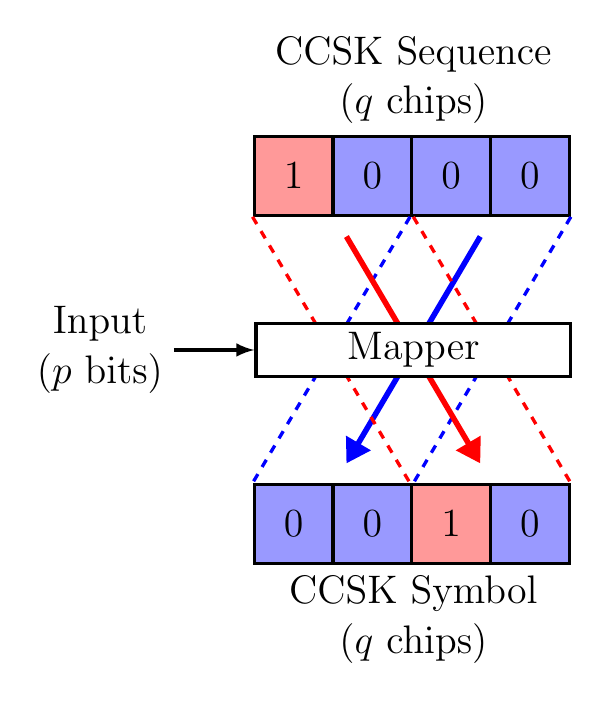
\begin{tikzpicture} [-latex,
    >=latex,
    auto,
    very thick,
    every node/.style={font={\Large}},
    main node/.style={rectangle, fill = white!35, draw,
        align=center}
  ]

  \node [main node,
    fill = red!40!white,
    minimum size = 1cm
  ] (ccsk0) at (0, 0)   {$1$};
  \node [main node,
    fill = blue!40!white,
    minimum size = 1cm
  ] (ccsk1) at (1cm, 0) {$0$};
  \node [main node,
    fill = blue!40!white,
    minimum size = 1cm
  ] (ccsk2) at (2cm, 0) {$0$};
  \node [main node,
    fill = blue!40!white,
    minimum size = 1cm
  ] (ccsk3) at (3cm, 0) {$0$};


  \node [main node,
    draw = none,
    minimum size = 1cm,
    anchor=north east,
    align = center
  ] (in) at ($(ccsk0.south west) + (-1,-1)$) {Input\\($p$ bits)};


  \node [main node,
    fill = blue!40!white,
    anchor=north west,
    minimum size = 1cm
  ] (symb0) at ($(in.south east)    + (1,-1)$) {$0$};
  \node [main node,
    fill = blue!40!white,
    minimum size = 1cm,
    anchor=north east,
  ] (symb1) at ($(symb0.north east) + (1, 0)$) {$0$};
  \node [main node,
    fill = red!40!white,
    minimum size = 1cm,
    anchor=north east,
  ] (symb2) at ($(symb1.north east) + (1, 0)$) {$1$};
  \node [main node,
    fill = blue!40!white,
    minimum size = 1cm,
    anchor=north east,
  ] (symb3) at ($(symb2.north east) + (1, 0)$) {$0$};

  \draw [blue, -, dashed] (ccsk2.south west) -- (symb0.north west);
  \draw [blue, -, dashed] (ccsk3.south east) -- (symb1.north east);
  \draw [blue, -Triangle,line width = 2pt] ($(ccsk2.south east) + (-.15, -.25)$) -- ($(symb0.north east) + (.15, .25)$);
  \draw [red, -, dashed] (ccsk0.south west) -- (symb2.north west);
  \draw [red, -, dashed] (ccsk1.south east) -- (symb3.north east);
  \draw [red, -Triangle,line width = 2pt] ($(ccsk0.south east) + (.15, -.25)$) -- ($(symb2.north east) + (-.15, .25)$);


  \node [main node,
    minimum width = 4cm,
  ] (map) at (ccsk1.east |- in.west) {Mapper};

  \draw (in.east) -- (map.west);

  \node[anchor = south, align = center] at (ccsk1.north east) {CCSK Sequence\\($q$ chips)};
  \node[anchor = north, align = center] at (symb1.south east) {CCSK Symbol\\($q$ chips)};

\end{tikzpicture}
\end{document}
